\documentclass[polish]{beamer}

% --- Pakiety -------------------------------------------------------

\usepackage[T1]{fontenc}
\usepackage[polish]{babel}
\usepackage{amsmath, mathtools, amssymb}
\usefonttheme{professionalfonts} % Włącza oryginalne fonty LaTeXa w matematyce
\usepackage{xcolor} % Pakiet do definiowania kolorów
\definecolor{bordowy}{RGB}{180, 0, 0} % Bordowy w modelu RGB
\usepackage[ruled,vlined]{algorithm2e}
\usepackage{hyperref}
\usepackage{lipsum}

% --- Użyteczne ustawienia -------------------------------------------

\usetheme{Berkeley}
\usecolortheme{beaver}

\setbeamertemplate{navigation symbols}{} 

\setbeamercolor{block title}{bg=gray!40, fg=bordowy} % Czerwony tytuł z białym tekstem
\setbeamercolor{block body}{bg=gray!15,fg=black} % Szare tło treści z czarnym tekstem

% --- Ustawienia bibliografii ----------------------------------------

  \setbeamertemplate{bibliography item}[text]
  \setbeamercolor*{bibliography entry author}{parent=black}
  \setbeamercolor*{bibliography entry location}{parent=black}
  \setbeamercolor*{bibliography item}{parent=black}
  \setbeamercolor*{bibliography entry note}{parent=black}


% --- SIDEBAR --------------------------------------------------------
\makeatletter
\setbeamertemplate{sidebar left}{
  \insertverticalnavigation{\beamer@sidebarwidth}%
  \vfill
}
\makeatother


% --- PRZESUNIECIE DLA STRONY TYTULOWEJ -----------------------------
\makeatletter
\newlength{\szerokoscSlide}
\setlength{\szerokoscSlide}{\paperwidth}
\addtolength{\szerokoscSlide}{-2cm} % Zmniejszamy o 2cm, zeby box z tytułem
% nie zajmowal calej szerokosci
\newcommand{\startodkrawedzi}{
  \hspace*{-\beamer@sidebarwidth}% Cofnij o szerokość paska bocznego
  \hspace*{-\beamer@leftmargin}% Cofnij o domyślny margines tekstu
}
\makeatother


% --- Dolny pasek ----------------------------------------------------
\setbeamertemplate{footline}{%
  \leavevmode%
  \hbox{%
      \begin{beamercolorbox}[wd=.5\paperwidth,ht=2.5ex,dp=1.1ex,right]{author in head/foot}%
      \insertshortauthor\hspace{1.2em}
    \end{beamercolorbox}%
    \begin{beamercolorbox}[wd=.43\paperwidth,ht=2.5ex,dp=1.1ex,left]{title in head/foot}%
      \hspace{1.2em}\insertshorttitle
    \end{beamercolorbox}%
  }%
  \begin{beamercolorbox}[wd=.07\paperwidth,ht=2.5ex,dp=1.1ex,center]{date in head/foot}%
\insertframenumber/\inserttotalframenumber
\end{beamercolorbox}%
  \vskip0pt%
}

% --- KOLORY sidebara -----------------------------------------------
\setbeamercolor{sidebar canvas}{bg=gray!15}
\setbeamercolor{section in sidebar}{fg=bordowy,bg=gray!15}
\setbeamercolor{section in sidebar shaded}{fg=black!45,bg=gray!15}
\setbeamercolor{subsection in sidebar}{fg=bordowy,bg=gray!15}
\setbeamercolor{subsection in sidebar shaded}{fg=black!45,bg=gray!15}

% --- Wygląd numeracji w spisie treści ------------------------------
\setbeamertemplate{section in toc}{%
  {\color{bordowy}\large$\bullet$}\hspace{0.6em}\inserttocsection\par
}
\setbeamertemplate{subsection in toc}{%
{\hspace{1em}\color{bordowy}\large$\bullet$}\hspace{0.6em}\inserttocsubsection\par
}


% --- Dane do prezentacji -------------------------------------------

\title[Jak przyspieszyć program]{Jak przyspieszyć program bez zmienia
złożoności obliczeniowej?}
\author[Tymon Tumialis]{Tymon Tumialis}
\institute{Seminarium Koła Naukowego Data Science}
\date[2026]{2026}
\logo{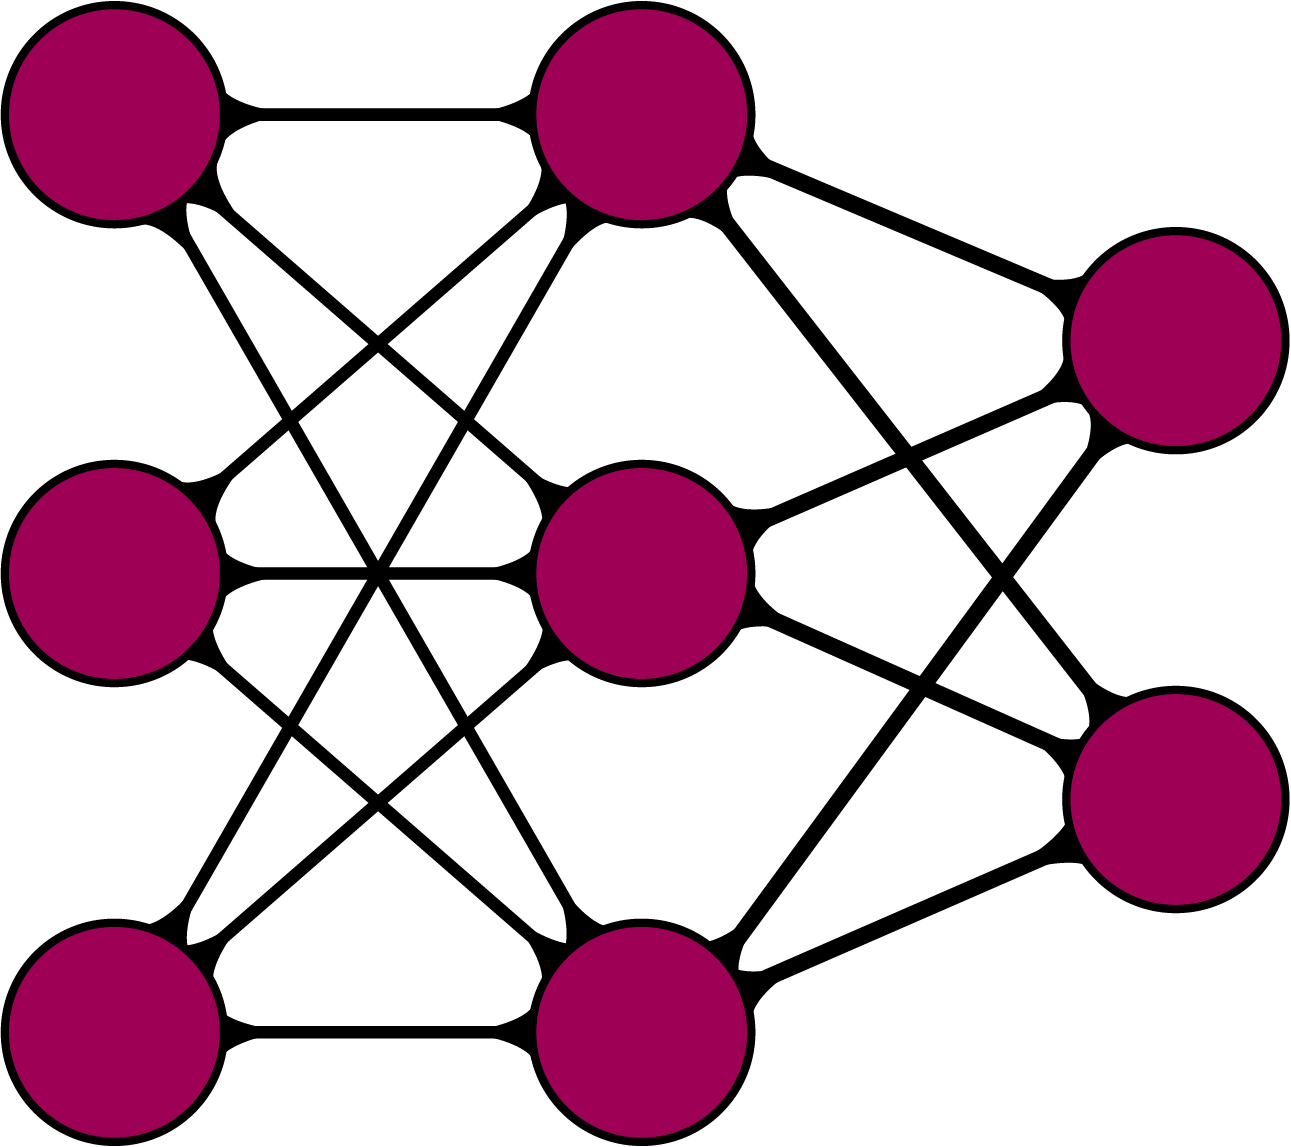
\includegraphics[height=1cm]{Graphics/KNDS_logo_bez_napisu.png}}

% --- Slajdy --------------------------------------------------------

\begin{document}

% Slajd tytułowy - nie zmieniać
\begin{frame}[plain]
  \startodkrawedzi
  \hspace{1cm} % Lewy margines
  \begin{minipage}[c][\textheight]{\szerokoscSlide}
    \centering
    \titlepage
    \vspace{-1cm} 
    \begin{figure}
      \centering
      
\includegraphics[width=0.4\textwidth]{Graphics/KNDS_logo_pełne.png}
      \hspace{2em}
      
\includegraphics[width=0.45\textwidth]{Graphics/politechnika.png}
    \end{figure}
  \end{minipage}
\end{frame}

% Spis treści 
\begin{frame}
\frametitle{Spis treści}
\tableofcontents
\end{frame}

% Slajdy warto dzielić na sekcje (section) i podsekcje (subsection).

%slajd 1
\section{Dlaczego szybki kod jest ważny?}

\begin{frame}{Dlaczego szybki kod jest ważny?}
  \begin{block}{Gdzie liczy się każda nano sekunda?}
    \begin{itemize}
      \item High Frequency Trading
      \item Programy do analizy wielkich zbiorów danych
      \item Algorytmy uczenia maszynowego
      \item Autonomiczne pojazdy
      \item Silniki do gier komputerowych
    \end{itemize}
  \end{block}

\end{frame}



% SLAJD 2
\section{Czy złożoności mówi nam wszystko o czasie wykonania?}
\begin{frame}{Czy złożoności mówi nam wszystko o czasie wykonania?}
   \begin{block}{Jest dobrą miarą, ale nie mówi nam wszystkiego}
    \begin{itemize}
      \item Przykładem jest przeiterowanie się po liście i tablicy. Złożoność teoretyczna O(N), ale różnica w czasie jest 10x
      \item Czas iteracji dla tablicy: 103 ms
      \item Czas iteracji dla vectora: 414 ms
      \item Czas iteracji dla listy: 1605 ms
      \item Dlaczego się tak dzieje?

    \end{itemize}
  \end{block}
\end{frame}

% SLAJD 3

\section{Piramida pamięci}

\subsection{Czym różni się L1 od RAM}
\begin{frame}{Najgorsze jest czekanie na dane}
    \begin{figure}
      \centering
      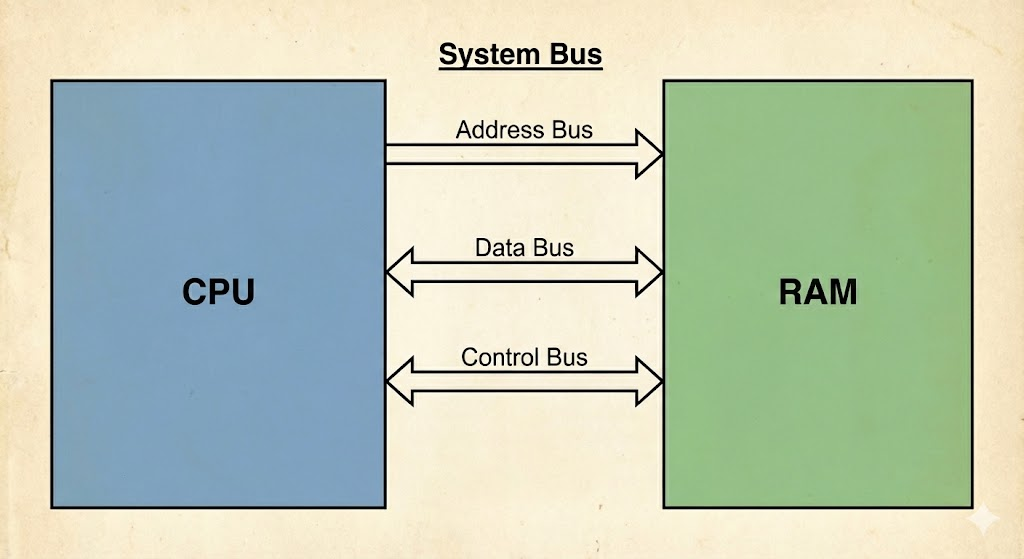
\includegraphics[width=0.8\textwidth]{Graphics/komunikacja_ram_cpu.jpg}
      \caption{\small komunikacja RAM CPU}
    \end{figure}


\end{frame}
% SLAJD 4
\begin{frame}{Czym jest cache?}
    \begin{figure}
      \centering
      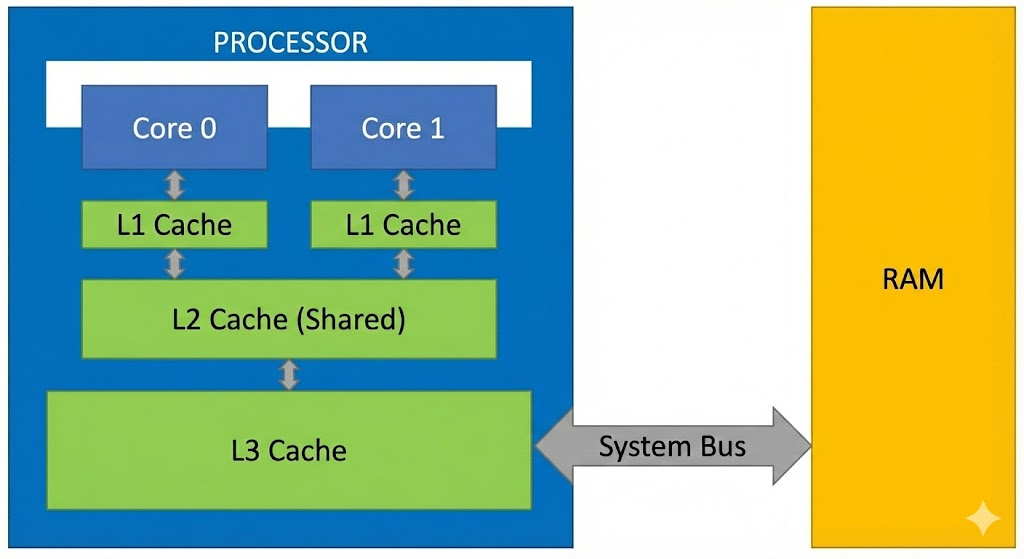
\includegraphics[width=0.8\textwidth]{Graphics/cpu_cache_ram.jpg}
      \caption{\small komunikacja RAM CPU z cachem}
    \end{figure}
    Cache to miejsce, w którym procesor trzyma często powtarzające się instrukcje.


\end{frame}

% SLAJD 5
\begin{frame}{Jak działa cache?}
    \begin{block}{Procesor jest sprytny}
    \begin{itemize}
      \item Patrzy czy instrukcja jest zapisana w cachu L1
      \item Jeżeli jest to ją wykonuje [nazywamy to cache hitem]
      \item Jeżeli nie ma jej w cachu to procesor ściąga ją z wyższych warstw pamięci [cach miss kosztuje nas czas]
      \item Procesor jest sprytny dlatego pobiera nie tylko jedną instrukcje tylko jej otoczenie, najczęscięj kolejne 64 bajty
      \item Robi to po to, żeby w kolejnym kroku uniknąć cache missu
    \end{itemize}
  \end{block}


\end{frame}

% SLAJD 6: 
\begin{frame}{Piramida pamięci}
    \begin{figure}
      \centering
      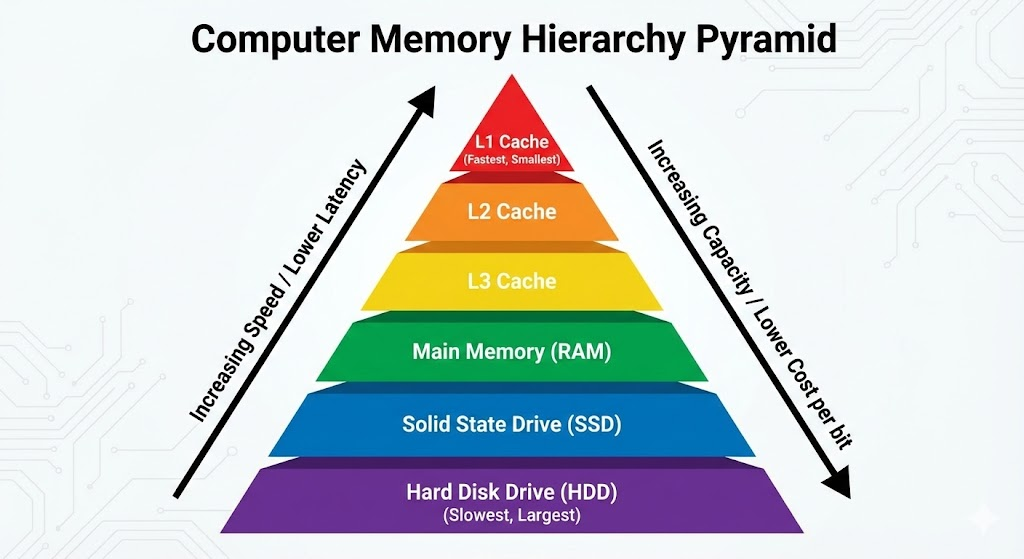
\includegraphics[width=0.8\textwidth]{Graphics/piramida_pamieci.jpg}
      \caption{\small piramida pamięci}
    \end{figure}


\end{frame}



% Slajd 7
\subsection{Liniowe struktury są najszybsze}
\begin{frame}{Lista vs Vector}

  \begin{block}{Przypomnienie czasu wykonania}
    \begin{itemize}
      \item Skupmy się na liście i vectorze
      \item Czas iteracji dla vectora: 414 ms
      \item Czas iteracji dla listy: 1605 ms
    \end{itemize}
  \end{block}


   \begin{block}{Różncia polega w sposobie trzymania danych w pamięci}
    \begin{itemize}
      \item Vector jest strukturą liniową - znaczy to, że zajmuje jeden duży blok pamięci
      \item Lista jest nie liniową strukturą danych - znaczy to, że jest porozrzucana w pamieci
    \end{itemize}
  \end{block}

\end{frame}

%Slajd 8

\begin{frame}{Wniosek}
Liniowe struktury danych są szybsze, ponieważ wykorzystują cache.

\begin{figure}
      \centering
      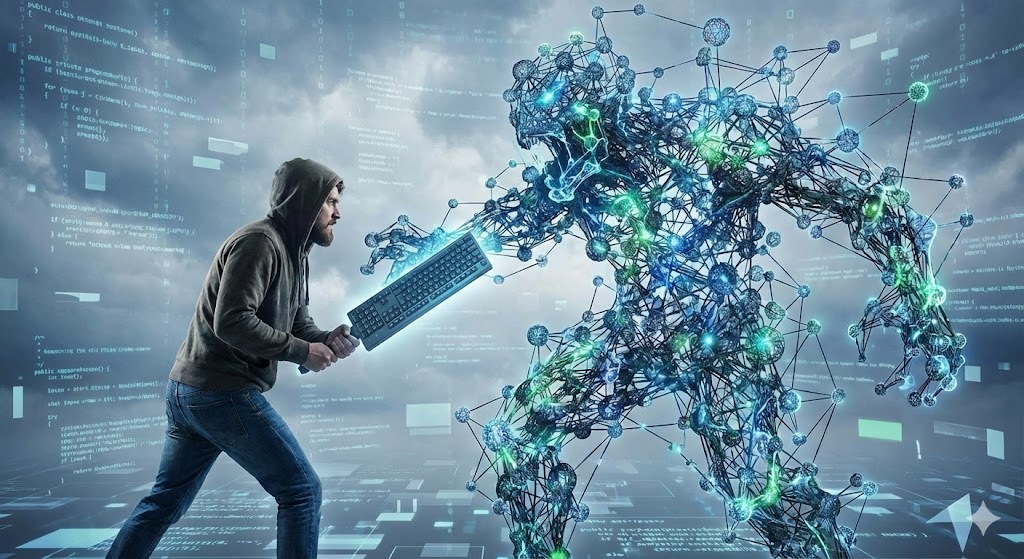
\includegraphics[width=0.8\textwidth]{Graphics/programista_vs_nodes.jpg}
      \caption{\small walka z nie liniowymi strukturami danych}
    \end{figure}
\end{frame}

%Slajd 9

\subsection{Stack vs Heap}
\begin{frame}{Ale dlaczego tablica jest 4x szybsza od vectora?}
   \begin{block}{Przypomnienie czasu wykonania}
    \begin{itemize}
      \item Skupmy się teraz na tablicy i vectorze
      \item Czas iteracji dla tablicy: 103 ms
      \item Czas iteracji dla vectora: 414 ms
    \end{itemize}
  \end{block}

  Różnica polega na tym, że tablica jest deklarowana na stosie [stack] a vector na stercie [heap].

\end{frame}


%Slajd 10

\subsection{Stack vs Heap}
\begin{frame}{Stack vs Heap}
   \begin{block}{Różnice między stackiem a heapem}
    \begin{itemize}
      \item Na stosie trzymamy dane o stałym rozmiarze
      \item Heap przechowuje dane, których rozmiar może się zmienić
      \item Żeby zaalokować nową pamięć na heapie musimy poprosić OS, żeby dał nam nowy chunk pamięci [wolne]
    \end{itemize}
  \end{block}

 \begin{block}{Dlaczego statyczna tablica jest szybsza?}
    \begin{itemize}
      \item Zapisywana na stosie
      \item Użuwa najprostszych instrukcji
    \end{itemize}
  \end{block}

\end{frame}



% SLAJD 11
\section{Pisanie dobrych ifów}
\subsection{Branch Predictor}
\begin{frame}{Branch Predictor}
  Zastanówmy się co się dzieje, gdy nasz program musi wykonać ifa.

  \begin{block}{Wyobraźmy sobie, że nasz program jest obsługiwany przez małe roboty}
    \begin{itemize}
      \item Robota, który sprawdza nasz warunek
      \item Robota, który próbuje przewidzeć jaka będzie kolejna instukcja po ifie
    \end{itemize}
  \end{block}

\end{frame}

%Slajd 12

\subsection{Upraszczanie ifów}
\begin{frame}{Wykorzystanie branch prediction}

  \small
    \begin{algorithm}[H]
        \SetAlgoLined
        code = function()
        \If{error 1}{
            obsługa..
        }
        \If{error 2}{
          obsługa..
        }
        \If{error 3}{
          obsługa..
        }
        \If{brak errora }{
          obsługa..
        }
        \caption{Obsługa błędów}
    \end{algorithm}


\end{frame}


% Slajd 13
\begin{frame}{Wykorzystanie branch prediction c.d}

  \small
    \begin{algorithm}[H]
        \SetAlgoLined
        code = function()
        \If{code == kod błedu}{
            obsługa..
        }
        \If{brak błedu}{
          obsługa..
        }
        \caption{Obsługa błędów lepsza}
    \end{algorithm}


\end{frame}


% SLAJD 14: Pseudokody

\subsection{Logika boola}
\begin{frame}{Logika boola}
  \begin{block}{Jak działa or i and}
    \begin{itemize}
      \item and jest prawdziwy jeżeli wszystkie warunki są prawdziwe
      \item or jest prawdziwy gdy co najmniej jeden warunek jest prawdziwy
    \end{itemize}
  \end{block}
Zastanówmy się czy kolejność wyrażeń w ifie ma znaczenie?



\end{frame}




% --- BIBLIOGRAFIA ---------------------------------------
\section{Koniec}
\begin{frame}{Koniec}
  Dziękuje za uwagę
\end{frame}

\end{document}